\documentclass[aspectratio=169,usenames,dvipsnames,10pt]{beamer}
\usetheme{HPC}
\setbeameroption{show only notes}


\begin{document}
	\input{TitleSlide}  	% TitleSlide
	\begin{frame}{Overview}
	\begin{enumerate}
		\item What is The Carpentries
		\item A Very Brief History of The Carpentries
		\item Where does HPC Carpentry fit?
		\item Current Status
		\item Roadmap and Challenges
		\item The mini version
		\item Comms Channels
	\end{enumerate}
	
	\note{What we will look at is what The Carpentries is about and how it came into existence. Most of you are probably quite familiar with it anyway so it will be very short. We'll then look at what HPC Carpentry is and how that came about. What the current status of the HPC Carpentries is and what our future plans are. I wouldn't be myself if I didn't squeeze a bit of the miniHPC in here, so I'll quickly mention that and then I'll leave you with ways to get into contact us so that you too can join us in brining HPC Carpentries to researchers.}	
\end{frame}

				% Overview
	\begin{frame}{A Very Brief History of The Carpentries}
	\begin{columns}[T]
		\begin{column}[c]{.5\textwidth}
			\begin{itemize}
				\item Software Carpentry was founded in 1998 with the mission of teaching lab skills for research computing by 
				Greg Wilson and Brent Gorda.
				\item HPC Carpentry making an appearance in ~2013
				\item Since then several presentations and workshops
				\item Formally accepted to Lesson Program Incubation, June 2023
			\end{itemize}
		\end{column}

		\begin{column}[c]{.5\textwidth}
			\begin{figure}
				\centering
				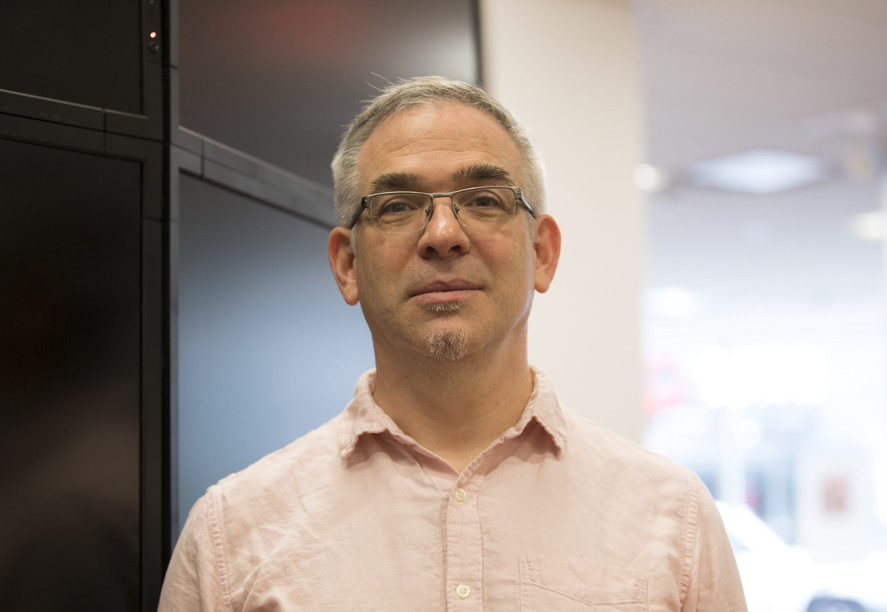
\includegraphics[width=.9\textwidth]{images/dr_greg_wilson.jpg} \linebreak
				\caption*{Dr Greg Wilson\linebreak\tiny\url{https://carleton.ca/scs/?p=14196}}
			\end{figure}
		\end{column}
	\end{columns}
	
	\note{It all started back in 1998 with Greg Wilson.  }
\end{frame}
				% Greg Wilson and Software Carpentries
	%	\begin{frame}{Where does HPC Carpentry fit?}
	\begin{enumerate}
		\item Knowing about version control and functions does not quite solve all problems.
		\item Researchers with HPC requirements do not necessarily know how to effectively scale their applications
		\item HPC facility operators become frustrated by non-knowledgable users making use of shared resources.
		\item Solution: Use Carpentries techniques.
	\end{enumerate}
		\note[item]{So once you write using functions and your code is in GitHub, you try running it on an HPC and you might find it runs a bit faster because it just so happens that the login node has a better spec than your average laptop or desktop. But people start yelling at you for running stuff on the login node and you don't know what the problem is because you've never heard about the Slurm scheduler thing and you neither does MPI sound familiar}
	\note[item]{Using the Carpentries' style and pedagogy we HPC Carpentry address this problem}
\end{frame}

\begin{frame}{How did it all begin}
	\begin{itemize}
		\item Earliest commit to hpc-carpentry GitHub 2013 by Compute Canada
		\item Peter Steinbach blog post (2017) - HPC in a day
		\item CarpentryCon 2018, 2020, 2022
		\item Super Computing BoF 17, 18, 19, 21
		\item Winter 2021, accepted into Carpentries Incubator
		\item Begin working towards Lesson Program Incubation in 2021 and formally accepted to the Lesson Program Incubation in June 2023
		\item April 2024, workflow lessons enters testing
		
	\end{itemize}
	\note[item]{The earliest commit I could find in the hpc-carpentry organisation was 2013. I watched a recording of a presentation given by Andrew Reid at SIGHPC about a year ago to get an idea of the history of HPC Carpentry and these were some of the events that Andrew mentioned that were significant in the spread of the word of HPC Carpentry, by talking to people, running workshops and getting feedback.}
\end{frame}



\begin{frame} {Where are we now?}
	\begin{enumerate}
		\item We are doing things In the Carpentries Way
		\begin{itemize}
			\item two day setting
			\item students type along with instructors
			\item get feedback
		\end{itemize}
		\item Two main takeaways:
			\begin{itemize}
				\item muscle memory 
				\item vocabulary
			\end{itemize}
		\item Not experts after two days but:
			\begin{itemize}
				\item know what answer looks like
				\item know how to find answers
			\end{itemize} 
	\end{enumerate}
	
	\note[item]{}
\end{frame}				% Where does HPC Carpentries fit?
	\begin{frame}{Current Status}
	\begin{itemize}
		\item We used to have our own shell lesson but that has now been deprecated in favour of the Software Carpentry lesson.
		\item HPC Intro has been reworked
		\item Using Amdahl executable rather than having students write and compile it
		\item There are two workflow management lessons available, for Snowflake and  Maestro
	\end{itemize}
\note{}
\end{frame}				% Current Status Curriculum
	\begin{frame}{Current Status: Lesson Support}
	\begin{itemize}
		\item Instructor Onboarding documentation available
		\item Lesson Maintainers onboarded by The Carpentries
		\item Infrastructure support allows customisation of lessons to reflect local cluster configurations
	\end{itemize}
	\note{}
\end{frame}

				% Current Status Lesson Support
	
\begin{frame}{Current Status: Community}
	\begin{itemize}
		\item Welcomed many new members to regular community calls + Maintainer teams
		\item Gathered interest in teaching+hosting workshops from the wider Carpentries community
		\item Completed Steering Committee elections
	\end{itemize}
	\note{}
\end{frame}				% Current Status Community
	\input{S7}				% Current Status Lesson Program Adoption
	\begin{frame}{Running Workshops}
	\begin{itemize}
		\item Workshops since January 2025
			\begin{itemize}
				\item NIST -- 2
				\item Newcastle -- 5
			\end{itemize} 
		\item Feedback to improve lesson infrastructure for adaptation to a specific HPC
		\item Snippets
		\item Episode on array jobs now included
		\item Onboarding for instructors
	\end{itemize}
	
\end{frame}				% Lesson adaption and workshops
	\begin{frame}{A miniHPC - CarpentriesOffline}
	\begin{columns}[T]
		\begin{column}[c]{.6\textwidth}
			\begin{itemize}
				\item Pixie: Raspberry Pi 4s, one login node, five compute nodes, one access point
				\item The same open source software stack as many HPCs: Slurm, lmod, munge
				\item Running Workshops and Hackerthons
					\begin{itemize}
						\item Lesson to build a login node and a compute node
						\item Adapt HPC lesson for Pixie
						\item Networking lesson
					\end{itemize}				
			\end{itemize}
		\end{column}
		
		\begin{column}[c]{.5\textwidth}
			\begin{figure}
				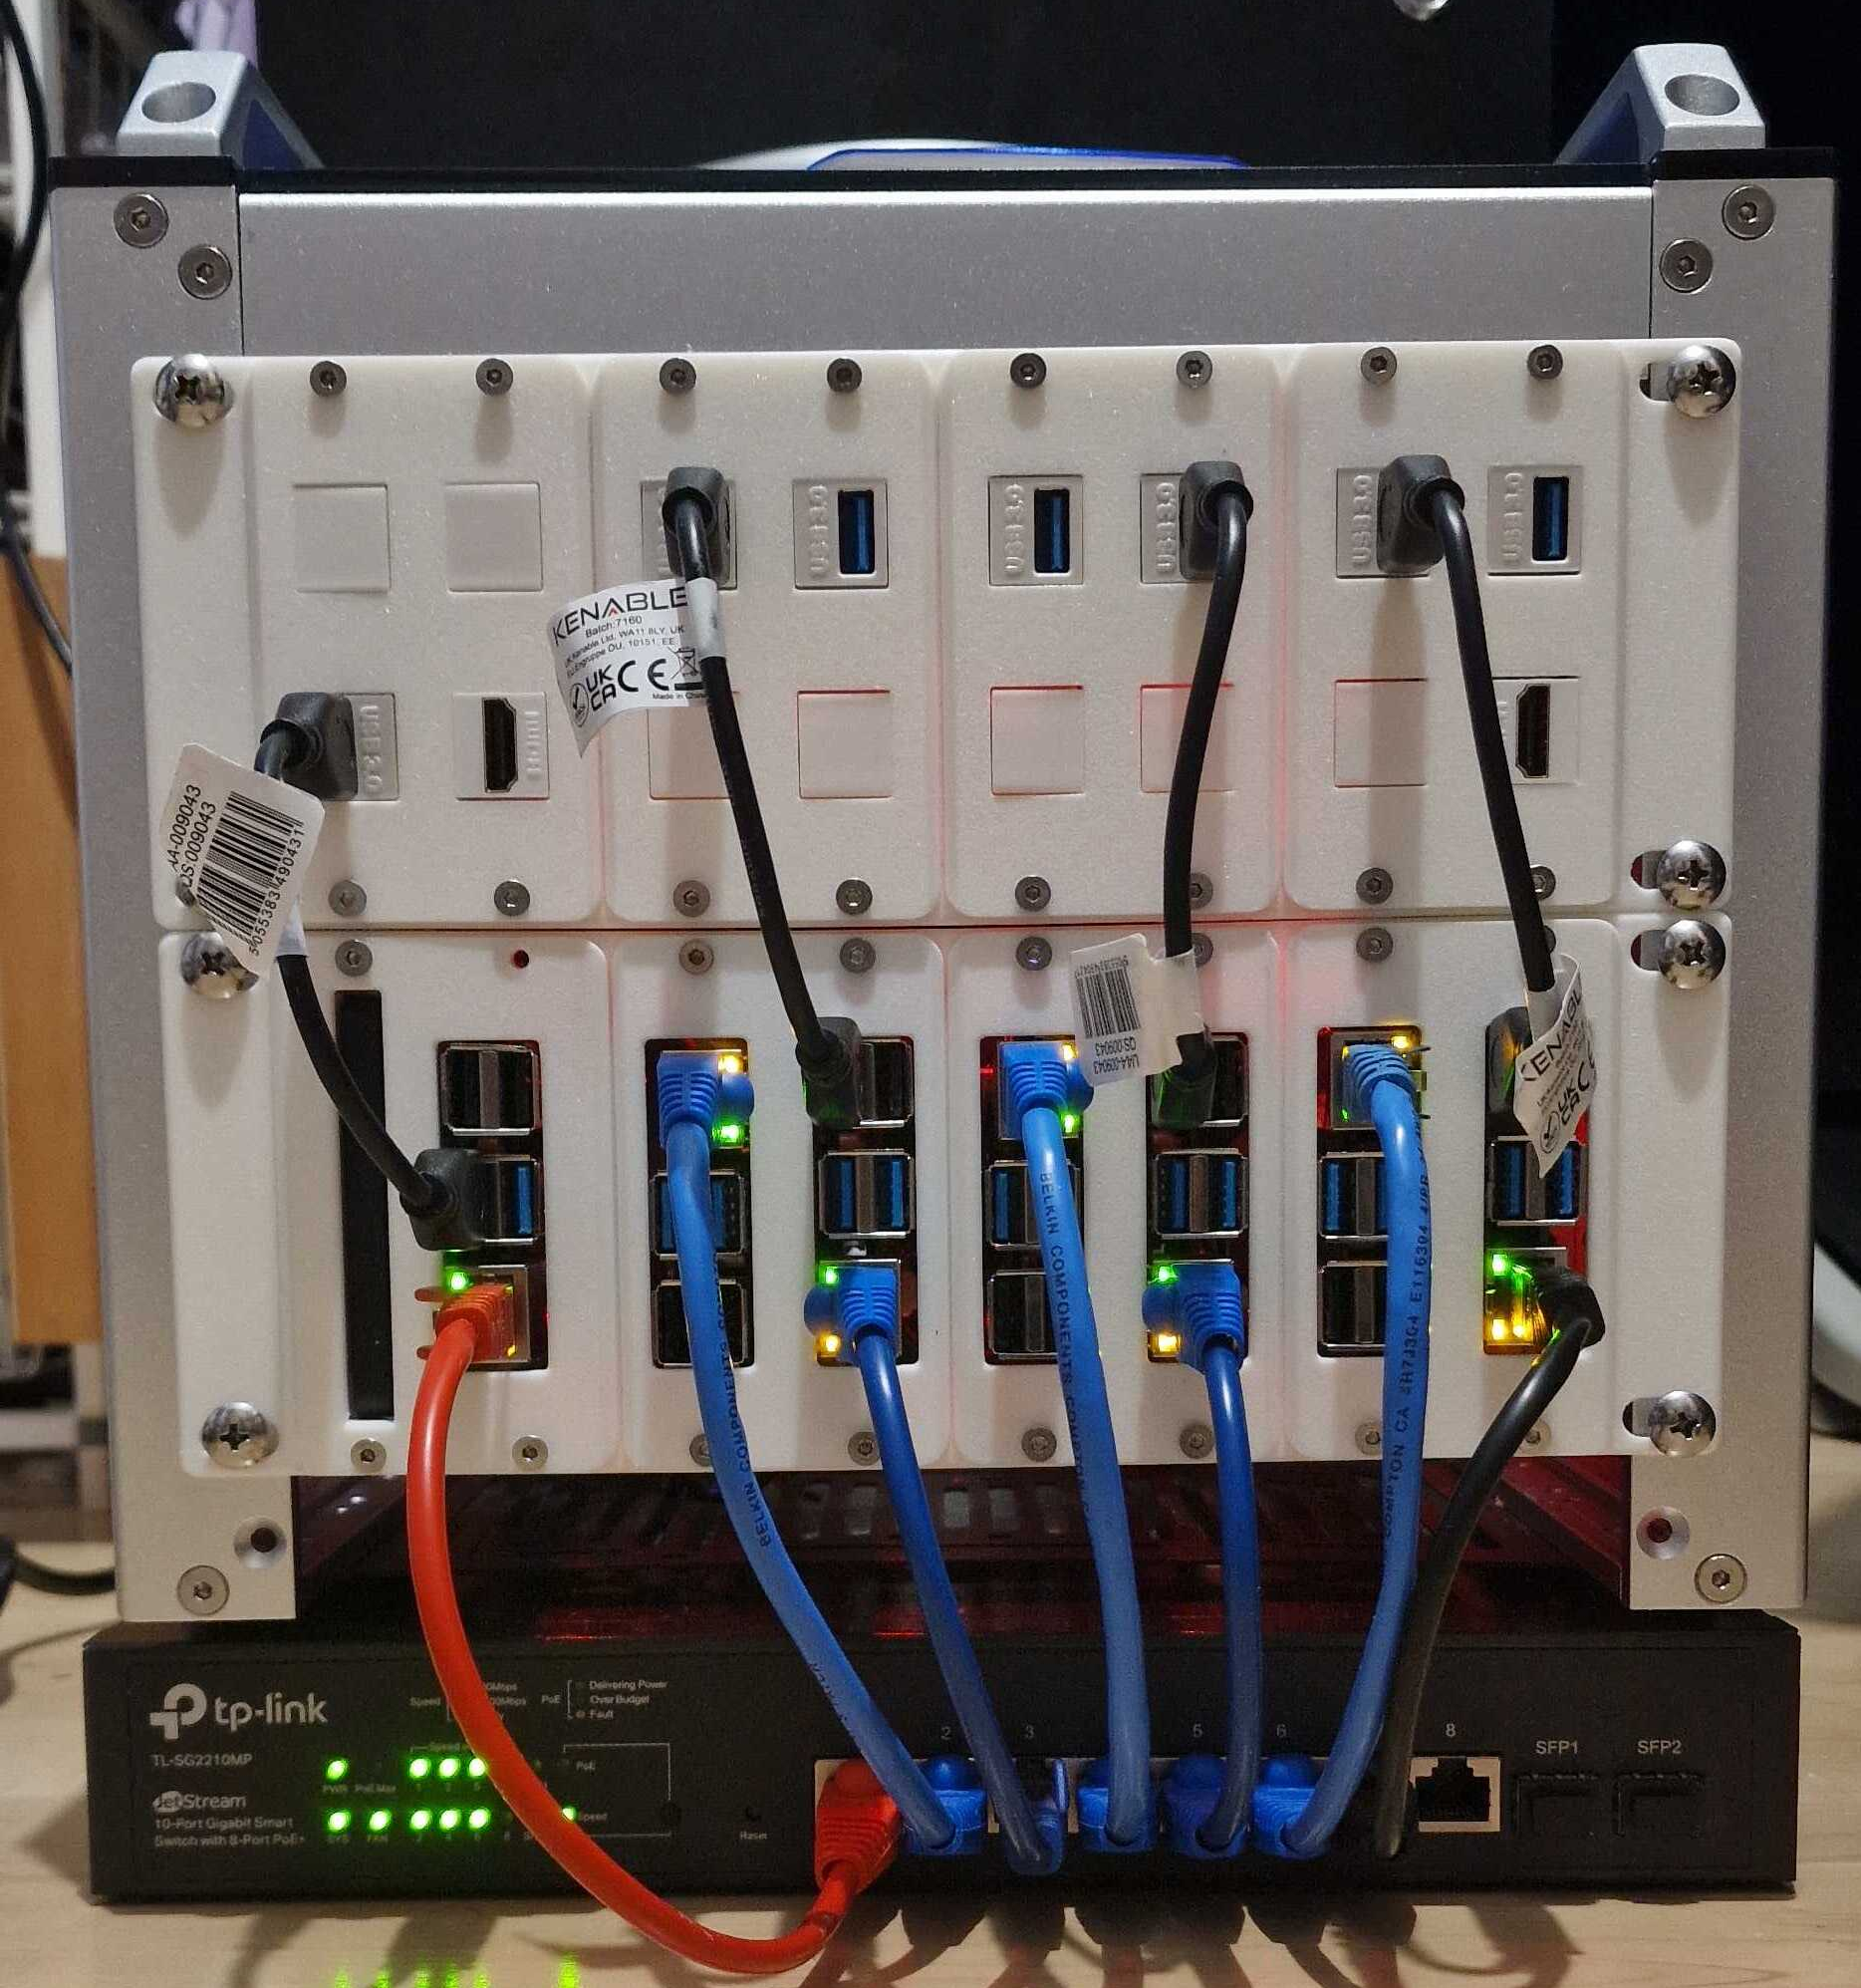
\includegraphics[width=.4\columnwidth]{images/mini-HPC-proto3.png} 
				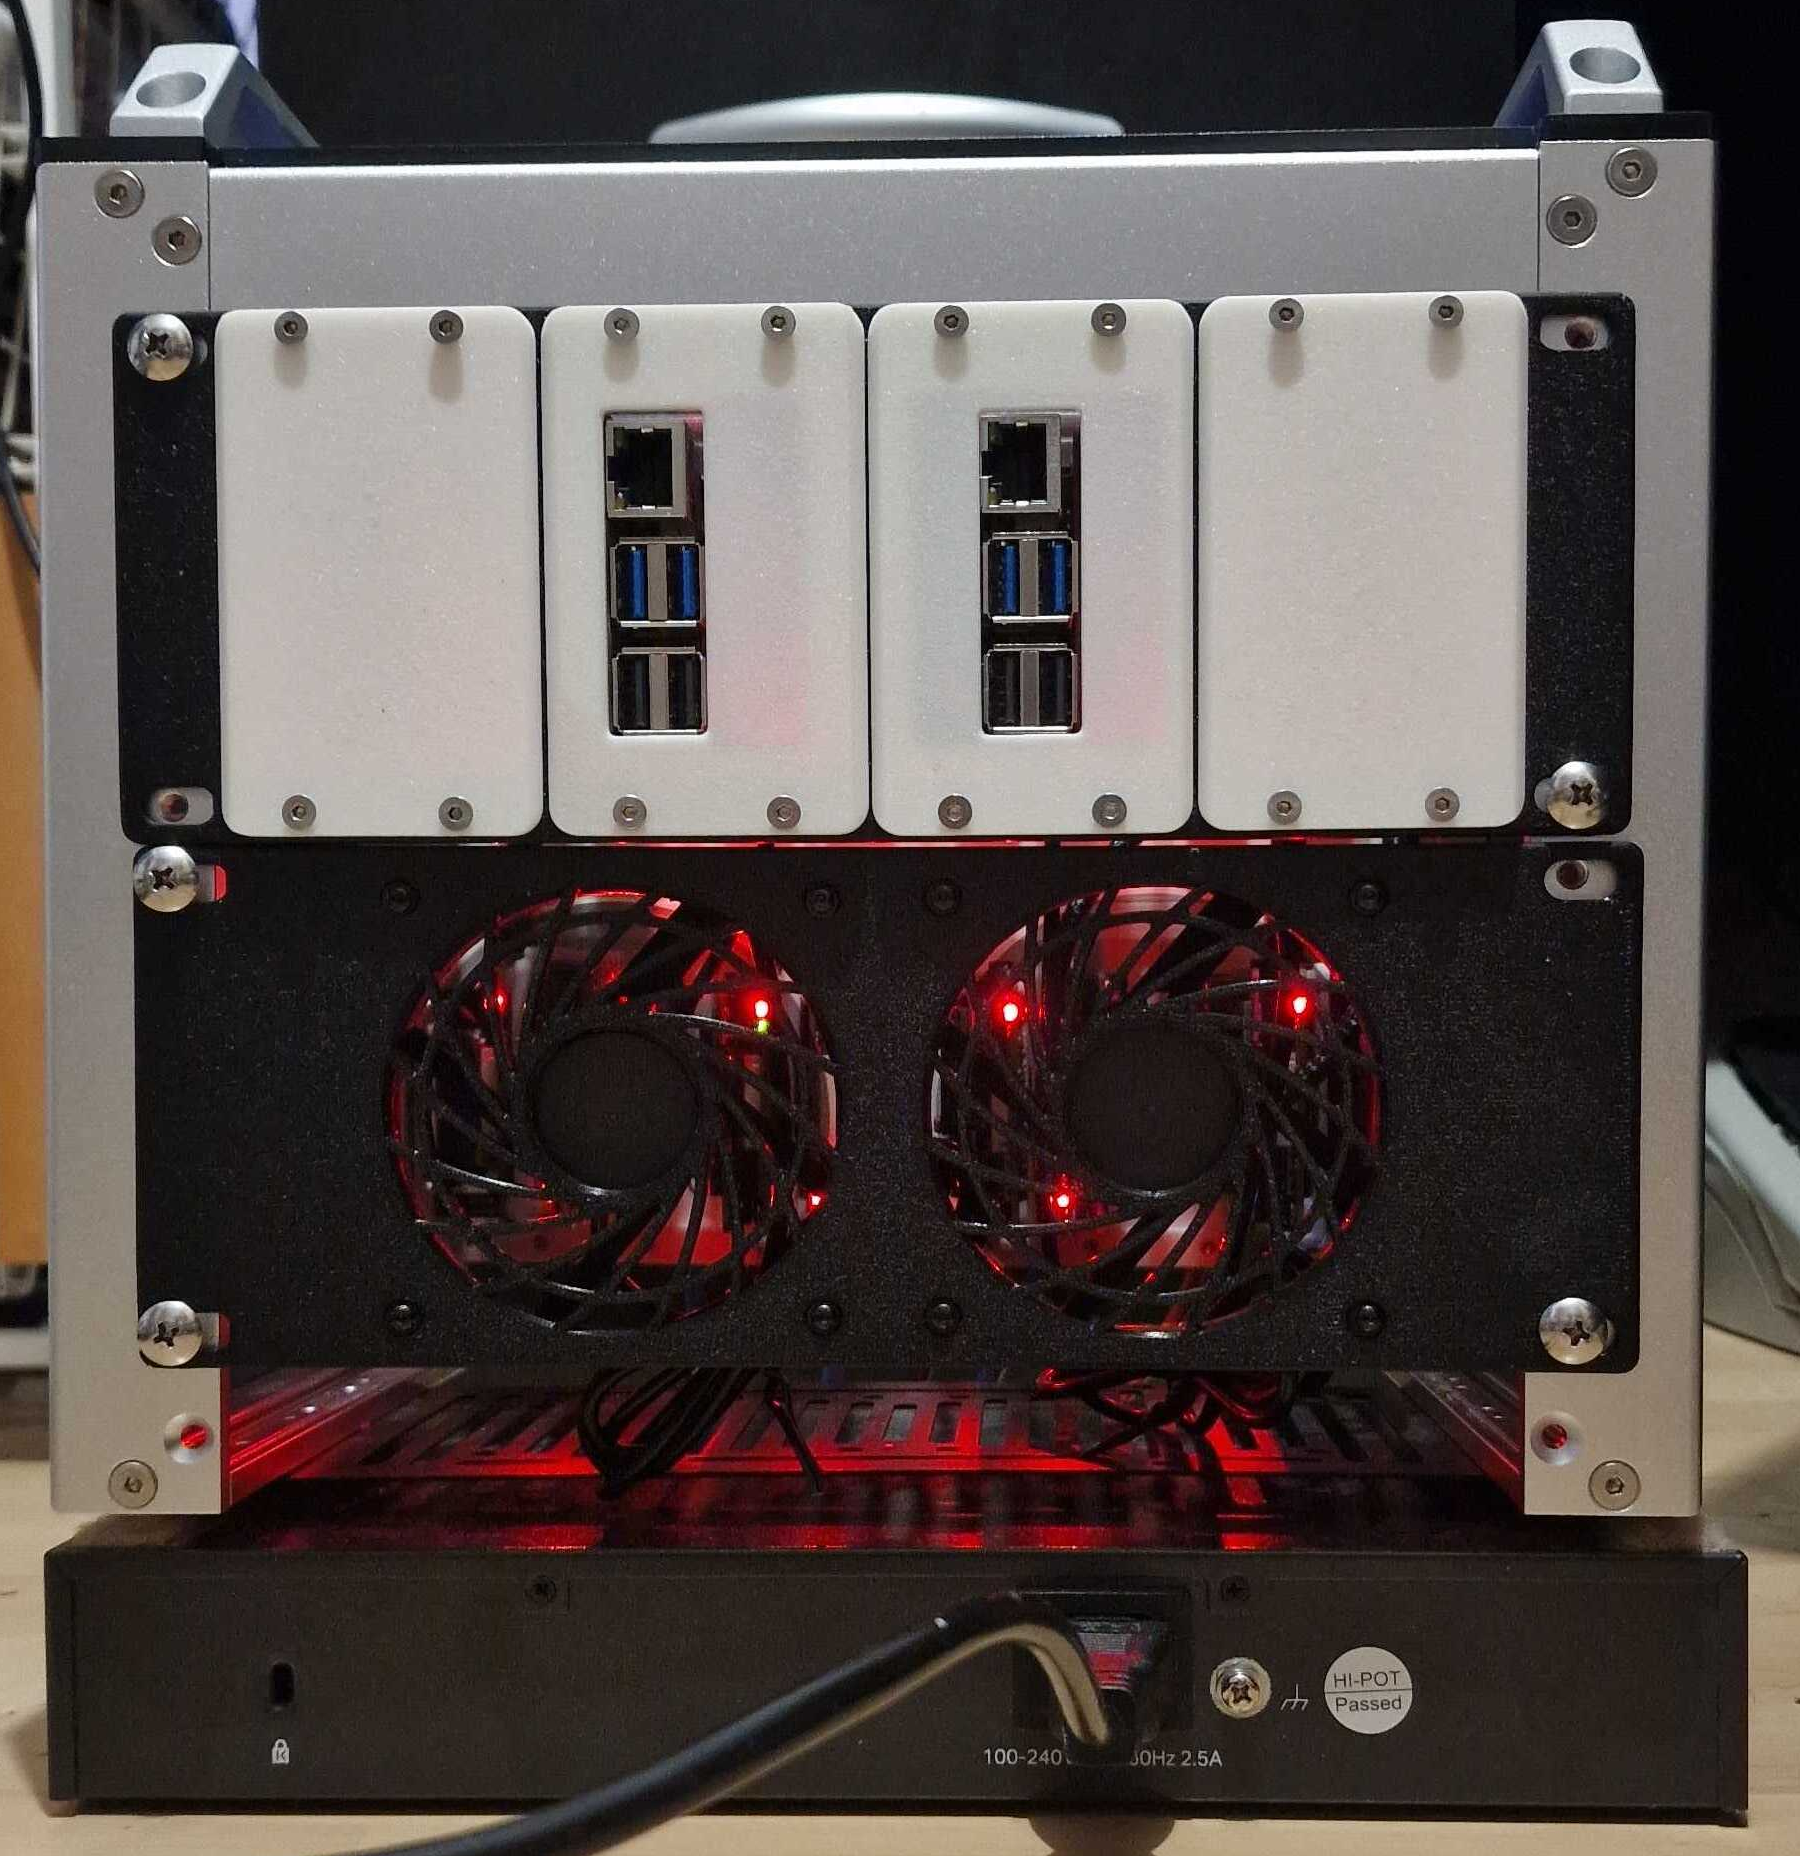
\includegraphics[width=.4\columnwidth]{images/mini-HPC-proto3_back.png}
				\caption*{Front and Back}
			\end{figure}
			\vspace{-2em} 
			\begin{figure}
				
\includegraphics[width=.2\columnwidth]{images/logo.png} 
			\end{figure}
		\end{column}
	\end{columns}
	
\end{frame}		% miniHPC
	\input{CommsChannels}	% Commns Channels
	\input{HelpNeeded} 		% Help Needed
	\begin{frame}{Resources}
	\begin{itemize}
		\item \textbf{Greg Wilson's talk at PyCon 2014} \url{https://www.youtube.com/watch?v=Wv0rf3Fyh7M}
		\item\textbf{ Andrew Reid's talk at SIGHPC 2024} \url{https://www.youtube.com/watch?v=FtKO619O5g0}
		\item\textbf{Peter Steinbach's blog post, HPC in a day?} \url{https://carpentries.org/blog/2017/06/hpccarpentry}
		\item\textbf{HPC Carpentry Website} 
		\url{https://www.hpc-carpentry.org}
		\item\textbf{CarpentriesOffline for the miniHPC}
		\url{https://carpentriesoffline.org}
		\item ChatGPT for its help with the \LaTeX \ template!
	\end{itemize}
\end{frame}		% Resources
\end{document}